\chapter*{Breve panoramica sulla libreria Py-Vicon}
\addcontentsline{toc}{chapter}{Breve panoramica sulla libreria Py-Vicon}

Questa libreria è quella che utilizziamo per ottenere dal Tracker le informazioni di posizione e orientazione di Drone e Wand. 
\\
Le uniche funzioni per noi di interesse sono quelle riportate nelle figure ~\ref{fig:getSegmentGlobalRotation} e ~\ref{fig:getSegmentGlobalTranslation}. 
\\
In realtà utilizzeremo anche una terza funzione che ci consente di recuperare l'informazione di orientazione di un oggetto tramite i relativi quaternioni. Questa funzione non è stata riportata in quanto come detto in precedenza il progetto allo stato attuale non "integra" alla perfezione l'utilizzo di questa funzione che sarebbe dovuta servire per aggiornare l'informazione di orientazione del drone nel suo filtro di Kalman. 
\\
\begin{figure}[h]
    \centering
    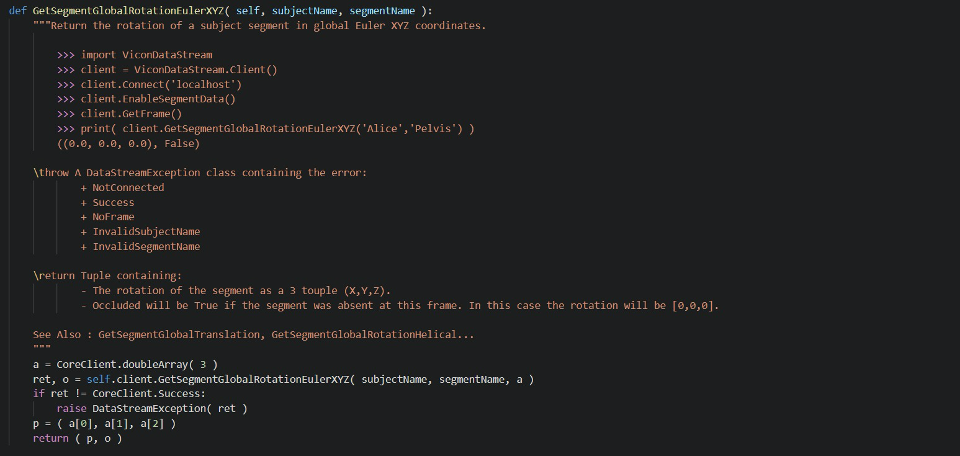
\includegraphics[width=1 \textwidth]{Relazione/Immagini/getSegmentGlobalRotation.png}	
    \caption{Funzione utilizzata per ricevere dal Tracker la matrice di rotazione che rappresenta l'orientazione di un oggetto rispetto alla terna fissa Vicon}
    \label{fig:getSegmentGlobalRotation}
\end{figure}
\\
\begin{figure}[h]
    \centering
    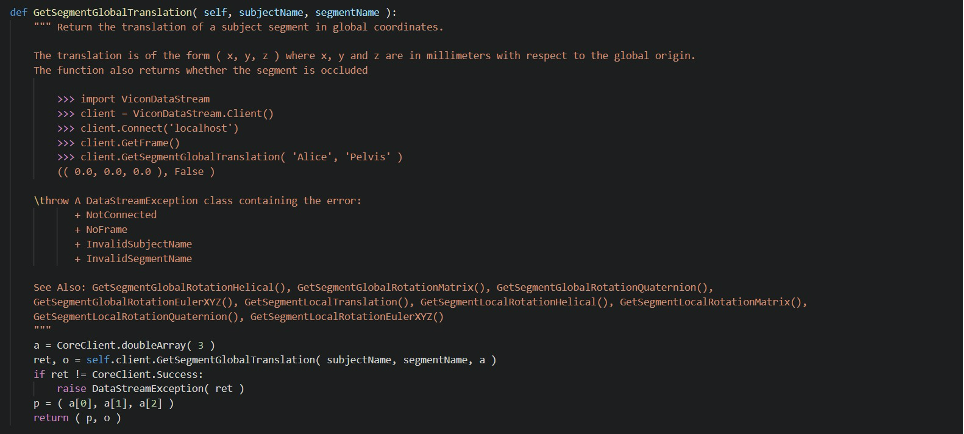
\includegraphics[width=1 \textwidth]{Relazione/Immagini/getSegmentGlobalTranslation.png}	
    \caption{Funzione utilizzata per ricevere dal Tracker il vettore posizione che rappresenta la traslazione dell'origine della terna Body di un oggetto rispetto all'origine della terna fissa Vicon, espressa nel sistema fisso Vicon}
    \label{fig:getSegmentGlobalTranslation}
\end{figure}
\\
\\
Queste funzioni restituiscono rispettivamente una struttura dati da cui poter ottenere facilmente la posizione \verb [x,y,z]  espressa in terna Vicon e la matrice di rotazione \verb (3x3)  risultante dalla composizione delle classiche rotazioni successive lungo gli assi \verb X-Y-Z  (secondo la parametrizzazione \verb "RPY" ).  
\\
\\
Il nostro scopo finale è riuscire ad inviare al Drone:

\begin{itemize}
    \item Riferimenti di posizione da inseguire utilizzando la \verb send_position_setpoint(x,y,z,0)  della classe \verb Commander .
    La posizione dovrà essere espressa nella giusta terna. Lo zero finale è il campo relativo all’angolo di Yaw "desiderato" dell’orientazione del Drone. Vedremo più avanti nel dettaglio le motivazioni alla base di questa scelta.
    \item Informazioni sulla sua posizione attuale all’interno del sistema Vicon al fine di utilizzarle per l’aggiornamento del filtro di Kalman, anche queste inviate dopo averle espresse nella terna corretta. Questo verrà fatto utilizzando la \verb send_extpos(x,y,z) .
\end{itemize}

(Nella sezione successiva riporteremo con più dettaglio tutto quanto riguarda la parte dedicata ai sistemi di riferimento e le convenzioni adottate durante l’esperimento).


